\documentclass[12pt,a4paper]{article}
%\usepackage[in]{fullpage}
\usepackage[utf8x]{inputenc}
\usepackage{cite}
%\usepackage{listings}
\usepackage[usenames]{xcolor}
\usepackage{graphicx}
\usepackage{hyperref}
\usepackage{xr} % cross-reference across files
\usepackage{float} %for H positioning

\externaldocument[TUT-]{tutorial}

% start a new section on a new page
\let\stdsection\section
\renewcommand\section{\newpage\stdsection}

%\lstset{ %
%  basicstyle=\footnotesize,        % the size of the fonts that are used for the code
%  breakatwhitespace=true,          % sets if automatic breaks should only happen at whitespace
%  breaklines=true,                 % sets automatic line breaking
%  commentstyle=\color{gray},    % comment style
%  keepspaces=true,                 % keeps spaces in text, useful for keeping indentation of code (possibly needs columns=flexible)
%  language=bash                 % the language of the code
%}

% latest version of the mrfioc2 device support
\newcommand{\latestDriverVersion}{2.7.6}


%opening
\title{EVR Manual}
%\author{Sašo Skube, PSI}
\date{}

\begin{document}

\maketitle

%\begin{abstract}
%\end{abstract}

\tableofcontents

%\newpage

\section{Introduction}\label{sec:Introduction}
Event receiver is a part of a timing system. A timing system consists of an event generator (EVG), a series of event receivers (EVR), software controlling them and a timing network. EVG generates a series of events, which are delivered to EVRs through a timing network. Each EVR is configured to respond to specific events in various ways, including processing EPICS records and generating pulses, synchronized clock or custom signals on its outputs.

mrfioc2~\cite{git_mrfioc2} is an EPICS device support for the Micro Research Finland (MRF)~\cite{mrf} timing system. The mrfioc2 enables us to configure and use the event generators and event receivers in the timing system. It comprises of EPICS device support for MRF timing system and uses devlib2~\cite{devlib2} with additional kernel modules (eg. PCIe) for communication with the hardware. This project is a continued development from the original mrfioc2 driver~\cite{mrfioc2}.

The rest of this document describes the mrfioc2 device support in regards to the Event Receiver. EVR and its configuration is described, then instructions for starting a new IOC application for EVR are provided. The document continues with basic developer information for the mrfioc2 and ends with a short description of the EVR GUI. Some sections deal with PSI specifics. These are mostly simplifications in the deployment or build process for the mrfioc2 device support.

\section{Event Receiver}\label{sec:Event Receiver}
EVRs are available in various form factors, each supporting the same basic functionality (executing functions, manipulating DBus,...), but with different number of components (inputs, outputs,...). Each of the EVR components and functionalities is configurable by the user and is briefly described in the following sections.

The mrfioc2 contains all the template files needed to use the EVR in your IOC application\footnote{mrfioc2 files and folders overview is available in Section~\ref{sec:mrfioc2 organization}, the template and substitution files are described in Section~\ref{sec:Macros}
 %and instructions how to use them in your IOC application are available in Section~\ref{sec:PSI IOC startup}
 .}. The templates are included in the substitution file, which is in turn loaded by the IOC application (as it is common with any IOC application). 
It is recommended to use one of the existing EVR substitution files, available in \texttt{mrfioc2/PSI/example/*.subs}. If these are not suitable, user can adopt them to their needs.
An EVR substitution file consists of
\begin{itemize}
	\item an EVR form factor specific template. This template contains all the records describing EVR components (eg. inputs, outputs, pulsers, ...) available on a specific EVR form factor. It accepts macros that allow application specific configuration of these components. For example, through setting a correct macro, one can enable or disable selected output. The following is the EVR substitution file snippet using EVR-VME-230 form factor template. It shows how to disable front panel output 1 by substituting macro \texttt{FrontOut1-Ena-SP} with 0.
	\begin{verbatim}
	file "$(mrfioc2_TEMPLATES=db)/evr-vme-230.db"
	{
	  {
	    .....
	    FrontOut1-Ena-SP=0,
	    .....
	  }
	}
	\end{verbatim}
	\item other templates, such as \texttt{evr-pulserMap.template, evr-softEvent.template, evr-specialFunctionMap.template, evr-delayModule.template}. These are used to define application specific behavior, such as mapping of events (described in Section~\ref{sec:Event mapping}) or defining additional components plugged in to the EVR (eg. universal I/O modules). 
\end{itemize}
Each of the example EVR substitution files in \texttt{mrfioc2/PSI/example} folder contains all the available macros for the form factor it represents, together with short documentation. Besides configuring the EVR by setting the appropriate macros in the EVR substitution file, it is also possible to configure the EVR through the GUI at runtime (starting the GUI is described in Section~\ref{sec:GUI}).


\paragraph{How to read this section:}
Each sub-section starts with a short description of an EVR component or functionality. It is followed by the description of available macros, that can be used in the EVR substitution file to configure the specific component or functionality of the EVR.
Macro name, its default value, a description, available settings with values or other important information regarding the configuration is listed.
\begin{quote}
Example: \textbf{macro name}=\emph{default value} : Description, with available settings. \texttt{Setting name (macro value)} or \texttt{important information} is emphasized.
\end{quote}
The exact number of form factor specific components is available in~\cite{mrm_evr}. 

\subsection{General configuration}
There is usually only one event receiver controlled from a single IOC application, though it is possible to configure more. Thus the name of the EVR and the system name it belongs to must be defined.

\paragraph{Substitution file macros}\footnote{For EVR form factors that support GTX outputs (more about these is available in~\cite{mrm_evr}), there is an additional macro. \textbf{ExtInhib-Sel}=\emph{0} is used to set whether to honor the hardware inhibit signal(\texttt{0}) or not (\texttt{1}).}
\begin{itemize}
\item
	\textbf{SYS}=\emph{MTEST-VME-EVRTEST} : The system name. 
\item
	\textbf{DEVICE}=\emph{EVR0} : The name of the connected Event Receiver / timing card, which should be the same as defined in the startup script of the IOC application. 
\end{itemize}

%For EVR form factors that support GTX outputs (more about these is available in~\cite{mrm_evr}), there is additional configuration option:
%\begin{itemize}
%\item
%	\textbf{ExtInhib-Sel}=\emph{0} : This macro takes effect only when
%configuring GTX ouputs on cPCI-EVRTG-300 form factor. Either honor
%the hardware inhibit signal(\texttt{0}) or don't care about hardware
%inhibit input state(\texttt{1}).
%\end{itemize}



\subsection{Events and event clock}\label{sec:Events and event clock}
EVR receives events transmitted by an event generator from the timing network. Event clock is the frequency, at which the events are transmitted. All the EVRs lock to the phase and frequency of the event clock, thus it is synchronized across the entire timing system.

\paragraph{Substitution file macros}
\begin{itemize}
\item
	\textbf{Link-Clk-SP}=\emph{124.916} : The event receiver requires a
reference clock to be able to synchronize on the incoming event
stream sent by the event generator. For flexibility, a programmable
reference clock is provided to allow the use of the equipment in
various applications with varying frequency requirements. It must be
close enough to the EVG clock to allow phase locking with
EVR. Available values are \texttt{50~MHz - 150~MHz}. 
%The clock reference for the event receiver is generated on-board the event receiver using a fractional synthesizer.
%\item
%\textbf{Link-RxMode-Sel}=\emph{1} : Set whether the \texttt{DBus(0)} or
%\texttt{DBus + Data Buffer(1)} are sent downstream (to the timing network). Distributed bus (described in Section~\ref{sec:DBus}) bandwidth may be shared by transmission of a configurable size data buffer to up to 2 kbytes. When data transmission is enabled the distributed bus bandwidth is halved. 
\end{itemize}

\subsection{Pulse Generator - Pulser (Pul)}\label{sec:Pulser}
A pulse generator is able to output a configured pulse upon reception of an event.
\begin{figure}[H]
	\centering
	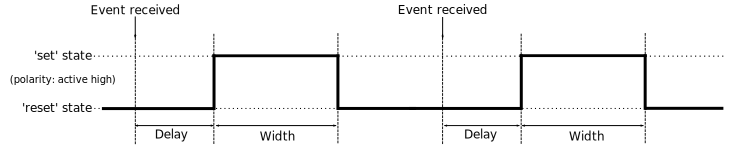
\includegraphics[width=\columnwidth]{./img/pulserGeneric}
	\caption{An example of a pulse generated after the reception of the event.}
	\label{fig:pulser_generic}
\end{figure}
Figure~\ref{fig:pulser_generic} shows how the pulse is generated by switching between set and reset states, where the states determine the logic level of the pulser output signal.

The pulser has configurable properties:
\begin{itemize}
	\item \textbf{Polarity} determines the logic level of the \texttt{set} and \texttt{reset} states. When polarity is set to
	\begin{itemize}
		\item \texttt{active high}, the \texttt{set state} puts the pulser output to logic high and the \texttt{reset state} puts the pulser output to logic low. 
		\item \texttt{active low}, the \texttt{set state} puts the pulser output to logic low and the \texttt{reset state} puts the pulser output to logic high.
	\end{itemize}
	\item  \textbf{Delay} determines the time from when the event was received to when the pulser enters the \textit{set state}.
	\item  \textbf{Width} determines the time from when the pulser enters the \textit{set state} to when it enters the \textit{reset state}.
\end{itemize}

Each received event can activate a function of the pulser:
\begin{itemize}
	\item \textbf{Trig} function uses polarity, delay and width to generate a pulse. Pulser starts in \texttt{reset state}. After the reception of an event, pulser waits \texttt{delay} ns and goes to \texttt{set state}. Then it waits for \texttt{width} ns and goes back to \texttt{reset state}.
	\item \textbf{Set} function puts the pulser to \texttt{set state}. Delay and width properties are ignored.
	\item \textbf{Reset} function puts the pulser to the \texttt{reset state}. Delay and width properties are ignored.
\end{itemize}

\paragraph{Substitution file macros}
There are a maximum of 24 pulsers available, depending on the EVR form factor. Pulsers are named Pul\#, where \# is the ID of the pulser ranging, from 0 to 23.
\begin{itemize}
  \item
    \textbf{Pul\#-Ena-Sel}=\emph{1} When \texttt{disabled(0)}, the output of the pulser will remain in its reset state. The pulser must be \texttt{enabled(1)} when used.
  \item
    \textbf{Pul\#-Polarity-Sel}=\emph{0} : Sets the pulser \textbf{polarity} to \texttt{active high(0)} or \texttt{active low(1)}.
  \item
    \textbf{Pul\#-Delay-SP}=\emph{0} : Sets the pulse \textbf{delay} in range of \texttt{0 us - 4294967295 us}.
  \item
    \textbf{Pul\#-Width-SP}=\emph{0} : Sets the pulse \textbf{width} in range of \texttt{0 us- 4294967295 us}. Maximum configurable width depends on the EVR form factor.
  \item
    \textbf{Pul\#-Prescaler-SP}=\emph{1} : Decreases the resolution of both \textbf{delay} and \textbf{width} by an integer factor. Value range: \texttt{0-65535}. Maximum configurable prescale value depends on the EVR form factor. Pulsers without prescalers use a fixed prescale value of 1.
  \end{itemize}
EVR-VME-300 also supports the following macros:
\begin{itemize}
  \item
    \textbf{Pul\#-Gate-Mask-SP}=\emph{0}: Set the gate (gates are described in Section~\ref{sec:Pulser gate}) used to mask this pulser. While the selected gate is activated, this pulser's \textbf{Trig} function is inhibited. Gates are selected using a bit mask, eg. value 0x1 corresponds to gate 0, value 0x2 corresponds to gate 1, value 0x3 corresponds to gate 0 and 1. Values are in range of \texttt{0x0 - 0xF}.
  \item
     \textbf{Pul\#-Gate-Enable-SP}=\emph{0}: Set the gate (gates are described in Section~\ref{sec:Pulser gate}) used to enable this pulser. While the selected gate is not activated, this pulser's \textbf{Trig} function is inhibited. Gates are selected using a bit mask, eg. value 0x1 corresponds to gate 0, value 0x2 corresponds to gate 1, value 0x3 corresponds to gate 0 and 1. Values are in range of \texttt{0x0 - 0xF}.
  \end{itemize}

\textbf{Substitution file macros} for mapping events to pulser function are available in Section~\ref{sec:Pulser mapping}, together with an \textbf{example}.

\subsubsection{Pulser gating (gates)}\label{sec:Pulser gate}
Pulser gating was introduced in series 300 of the event receivers. In EVR-VME-300 form factor, there exist 4 pulsers configured as gates (pulser 28 - pulser 31), which correspond to gate 0 - gate 3. They differ from normal pulser:
\begin{itemize}
	\item can only be enabled or disabled (\textbf{Pul\#-Ena-Sel}), where setting other properties has no effect.
	\item only uses \textbf{Set} and \textbf{Reset} functions, not the \textbf{Trig} function of the pulser.
\end{itemize}

\subsection{Outputs}\label{sec:Outputs}
\begin{figure}[H]
	\centering
	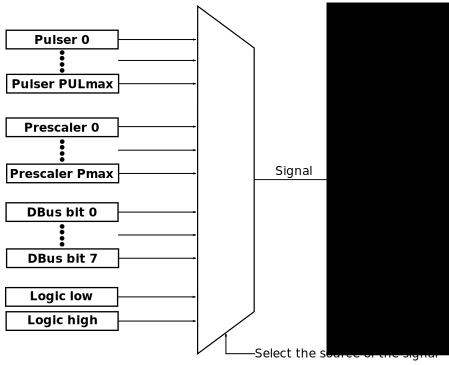
\includegraphics[]{./img/output}
	\caption{Available source signals for each output}
	\label{fig:output}
\end{figure}

An EVR has a number of outputs, each with a configurable source signal. As seen in Figure~\ref{fig:output}, any of the available pulser, prescaler, DBus, logic low or logic high signals can be selected as the output source signal. Depending on the output type(TTL, CML, ...), the signal can be send through directly, further manipulated or used as a trigger for a special function of that output.

\paragraph{Substitution file macros common to all outputs:} Outputs, and the corresponding macro name prefixes, are named either \emph{FrontOut\#},\emph{ FrontUnivOut\#} or \emph{RearUniv\#}, where the range of the number \# depends on the EVR form factor. Macros for the \emph{FrontOut0} are described below. 

\begin{table}[!hbt]
\caption{Output source signal mappings}
\label{tab:mappings}
\centering
	\begin{tabular}{|c|c|}
		\hline \textbf{mapping} & \textbf{output source} \\ \hline 
		\hline 0 & Pulser 0 \\ 
		\hline 1 & Pulser 1 \\ 
		\hline 2 & Pulser 2 \\ 
		\hline 3 & Pulser 3 \\ 
		\hline 4 & Pulser 4 \\ 
		\hline 5 & Pulser 5 \\ 
		\hline 6 & Pulser 6 \\ 
		\hline 7 & Pulser 7 \\ 
		\hline 8 & Pulser 8 \\ 
		\hline 9 & Pulser 9 \\ 
		\hline 10 & Pulser 10 \\ 
		\hline 11 & Pulser 11 \\ 
		\hline 12 & Pulser 12 \\ 
		\hline 13 & Pulser 13 \\ 
		\hline 14 & Pulser 14 \\ 
		\hline 15 & Pulser 15 \\ 
		\hline 16 & Pulser 16 \\ 
		\hline 17 & Pulser 17 \\ 
		\hline 18 & Pulser 18 \\ 
		\hline 19 & Pulser 19 \\ 
		\hline 20 & Pulser 20 \\ 
		\hline 21 & Pulser 21 \\
		\hline 22 & Pulser 22 \\
		\hline 23 & Pulser 23 \\
		\hline 32 & Distributed bus bit 0 \\ 
		\hline 33 & Distributed bus bit 1 \\ 
		\hline 34 & Distributed bus bit 2 \\ 
		\hline 35 & Distributed bus bit 3 \\ 
		\hline 36 & Distributed bus bit 4 \\ 
		\hline 37 & Distributed bus bit 5 \\ 
		\hline 38 & Distributed bus bit 6 \\ 
		\hline 39 & Distributed bus bit 7 \\ 
		\hline 40 & Prescaler 0 \\ 
		\hline 41 & Prescaler 1 \\ 
		\hline 42 & Prescaler 2 \\ 
		\hline 62 & Logic High \\ 
		\hline 63 & Logic low \\ 
		\hline 
	\end{tabular} 
\end{table}

  \begin{itemize}
  \item
   \textbf{FrontOut0-Ena-SP}=\emph{1} : When set to \texttt{enabled(1)} the mapping
    defined in \texttt{FrontOut0-Src-SP} is used. When \texttt{disabled(0)}, a
    mapping of \texttt{Force Low(63)} from Table~\ref{tab:mappings} is used.
  \item
    \textbf{FrontOut0-Src-SP}=\emph{63} : \texttt{Mappings} from the Table~\ref{tab:mappings} are
    set here. Any of the available pulser, prescaler, DBus, logic low or
    logic high signals can be selected as the output source signal.
  \end{itemize}
EVR-VME-300 also supports the following macros\footnote{EVR-PCIe-300 also supports this mechanics, but it was not tested}:
\begin{itemize}
  \item
    \textbf{FrontOut0-Src2-SP}=\emph{63} : Two sources for one output can be selected. The resulting output signal is a logical OR of \textbf{FrontOut0-Src-SP} and \textbf{FrontOut0-Src2-SP} source signals. As with \textbf{FrontOut0-Src-SP}, \texttt{mappings} from the Table~\ref{tab:mappings} are set here. Any of the available pulser, prescaler, DBus, logic low or logic high signals can be selected as the second output source signal.
  \end{itemize}
  
\subsubsection{Front Panel TTL Output (FrontOut)}\label{sec:Front Panel TTL Output}
These outputs are capable of driving TTL compatible logic level signals. The output source signal is converted to TTL logic levels(LVTTL of max 3.3 Volts) and send through the output, as seen in Figure~\ref{fig:output_ttl}.

\begin{figure}[H]
	\centering
	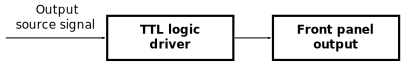
\includegraphics[]{./img/TTL}
	\caption{Front panel TTL output}
	\label{fig:output_ttl}
\end{figure}

\subsubsection{Front Panel CML Output (FrontOut)}\label{sec:Front Panel CML Output}
These outputs are capable of driving Current-mode logic compatible signals. Based on the output source signal and the selected CML mode, various patterns can be generated. As seen in Figure~\ref{fig:output_cml}, patterns are generated using one of the three configurable modes. They are sent out with a bit rate of \texttt{NBIT} times the event clock rate, thus the outputs allow for producing fine grained adjustable pulses and clock frequencies. Value of \texttt{NBIT} depends on the event receiver form factor (\texttt{NBIT} is 20 in EVR-VME-230 and 40 in EVR-VME-300).
\begin{figure}[H]
	\centering
	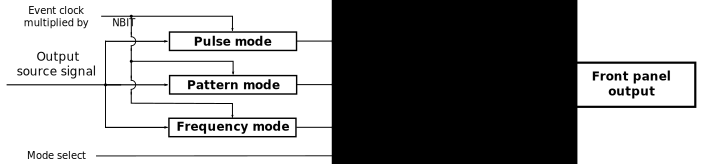
\includegraphics[width=\columnwidth]{./img/CML}
	\caption{Overview of the front panel CML outputs}
	\label{fig:output_cml}
\end{figure}

\paragraph{Substitution file macros} for general CML configuration:
There are a maximum of 8 CML outputs available, depending on the EVR form factor. CML outputs are named CML\#, where \# is the ID of the CML output, ranging from 0 to 7. Some form factors do not have any CML outputs.
\begin{itemize}
\item
  \textbf{CML\#-Ena-Sel}= \emph{0} : Output is \texttt{disabled(0)} or \texttt{enabled(1)}.
\item
  \textbf{CML\#-Pwr-Sel}=\emph{0} : Outputs can be \texttt{powered down(0)} or in normal \texttt{operation(1)}.
\item
  \textbf{CML\#-Rst-Sel}=\emph{0} : It is possible to \texttt{reset CML output(1)} or leave it in \texttt{normal operation(0)}.
\item
  \textbf{CML\#-Mode-Sel}=\emph{0} : There are three configurable modes, \texttt{pattern mode(0)}, \texttt{frequency mode(1)} and \texttt{waveform mode(2)}.
\end{itemize}
Patterns are defined by one of the configurable CML modes:
\begin{itemize}
\item 
	In \textbf{pulse mode} a user configurable \texttt{NBIT}-bit pattern is sent out based on the output source signal:
	
	\begin{itemize}
		\item
		  \textbf{rising edge}: pattern is sent out
		  after the rising edge is detected and will interrupt the current
		  pattern being sent.
		\item
		  \textbf{falling edge}: pattern is sent out
		  after the falling edge is detected and will interrupt the current
		  pattern being sent.
		\item
		  \textbf{logic high}: pattern is sent out after
		  the rising edge is detected and will repeat until the falling edge.
		\item
		  \textbf{logic low}: pattern is sent out after
		  the falling edge is detected and will repeat until the rising edge.
		\end{itemize}
	
\item 
	In \textbf{frequency mode} a clock signal can be generated. Its frequency is tuned in steps of \texttt{NBIT} times the event clock frequency.  The clock signal is synchronized by the output source signal(pulser, DBus signal, ....). 
	
	Frequency generation is triggered by a rising edge of the output source signal. After the trigger, it waits for a configured initial delay before it starts to generate a clock signal. 
		
	\paragraph{Substitution file macros}
	\begin{itemize}
	\item
	  \textbf{CML\#-Freq:Lvl-SP}=\emph{0} : set the starting logic level for the frequency generation. Options are:
	  \begin{itemize}
	  	\item \texttt{Active high(0)}: starting logic level is logic high
	  	\item \texttt{Active low(1)}: starting logic level is logic low
	  \end{itemize}
	\item
	  \textbf{CML\#-Freq:Init-SP}=\emph{0} : Set the initial delay between when the frequency generation is triggered and when it starts to generate a clock signal. This allows for a phase difference between the output source signal and the output signal. The value range in ns depends on the event clock. It must be in range of 1 event clock period to 3276 event clock periods.
	\item
	  \textbf{CML\#-Freq:High-SP}=\emph{10} : sets the amount of time in ns the signal stays on logic high, before switching to logic low. The value range in ns depends on the event clock. It must be in range of 1 event clock period to 3276 event clock periods.
	\item
	  \textbf{CML\#-Freq:Low-SP}=\emph{10} : sets the amount of time in ns the signal stays logic low, before switching to logic high. The value range in ns depends on the event clock. It must be in range of 1 event clock period to 3276 event clock periods.
	\end{itemize}
\item 
	In \textbf{pattern mode}, one can generate arbitrary bit patterns(waveforms), triggered by the output source signal(pulser, DBus signal,...). The waveform length is in multiple of \texttt{NBIT} bits (each bit is 1/\texttt{NBIT} of the event clock period), where maximum waveform length is \texttt{NBIT}x2048 bits.
	%	  \textbf{timeline} (\emph{Pat:WfX-I}): displays the times at which an  element from the pattern will be sent out.
		
	\paragraph{Substitution file macros}
	\begin{itemize}
	\item
	  \textbf{CML\#-Pat:WfCycle-SP}=\emph{0} : In \texttt{single shot mode(0)} the
	  waveform is sent only once per received trigger, where in \texttt{loop mode(1)}
	  the pattern will continuously loop after the first trigger occurred.
	\end{itemize}
	
	There is an additional delay calculator available to simplify waveform creation. 
	\paragraph{A delay calculator} has configurable \texttt{delay} and \texttt{width} macros to generate a pulse(similar to a pulser):
	\begin{itemize}
	\item
	  \textbf{CML\#-WfCalc:Ena-SP}=\emph{0} : \texttt{enable(1)} or \texttt{disable(0)} the calculation.
	\item
	  \textbf{CML\#-WfCalc:Delay-SP}=\emph{16} : can be used to specify the time in ns between when the mode is triggered and the pulse is generated. The value range in ns depends on the event clock. It must be in range of 1 event clock period to 2048 event clock periods.
	\item
	  \textbf{CML\#-WfCalc:Width-SP}=\emph{50} : can be used to specify the width of the pulse - the time the signal is stable at logic high. The value range in ns depends on the event clock. It must be in range of 1 event clock period to 2048 event clock periods.
	\end{itemize}
	
	%\paragraph{A bunch train calculator} that generates a series of consecutive pulses with width and delay fixed to $(event clock) / 4$. As seen in Figure~\ref{fig:output_cml_bunch}, each bunch pattern consists of \texttt{NBIT/2} %logic low bits and \texttt{NBIT/2} logic high bits. A bunch train always ends with \texttt{NBIT} logic low bits.
	%	\begin{figure}[H]
	%		\centering
	%		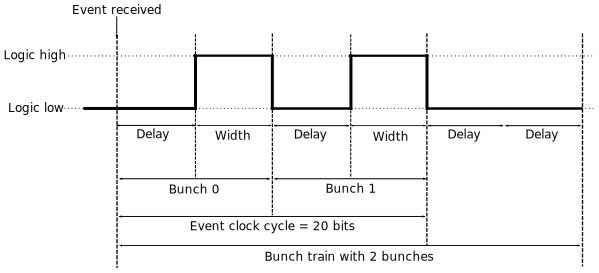
\includegraphics[width=0.96\columnwidth]{./img/bunchTrain}
	%		\caption{A bunch train example with 2 bunches when \texttt{NBIT=20}}
	%		\label{fig:output_cml_bunch}
	%	\end{figure}
	%	
	%	Bunch train calculator has the following substitution macros for configuration:
	%	\begin{itemize}
	%	\item
	%	  \textbf{CML\#-BunchTrain:Ena-SP}=\emph{0} : \texttt{enable(1)} or \texttt{disable(0)} the bunch train calculator
	%	\item
	%	  \textbf{CML\#-BunchTrain:Size-SP}=\emph{1} : set the number of bunches per train in range of \texttt{1-150}.
	%	\end{itemize}
	
\end{itemize}


\subsubsection{Front Panel Universal I/O (FrontUnivOut)}\label{sec:Front Panel Universal I/O}
Universal I/O slots provide different types of input or output with exchangeable Universal I/O modules~\cite{mrf_modules}. Each module provides two inputs or outputs (TTL, NIM or optical). 
The exact output signal is dependent on the inserted module. Figure~\ref{fig:output_univ}, shows an example of a universal I/O module with two outputs inserted in front panel universal slot.
\begin{figure}[H]
	\centering
	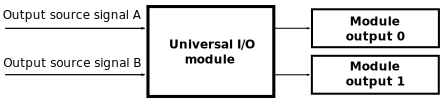
\includegraphics[]{./img/univ}
	\caption{An example universal I/O module with two outputs.}
	\label{fig:output_univ}
\end{figure}

\subsubsection{Rear Universal output - Transition Board output (RearUniv)}\label{sec:Rear Universal output}
An EVR has additional rear universal outputs. The exact output signal is dependent on the universal module inserted in the transition board.

\subsection{Event mapping}\label{sec:Event mapping}
As mentioned in Section~\ref{sec:Introduction}, an EVR responds to events. In order for the EVR to respond, an appropriate mapping between the event and  EVR function/component needs to be configured.

\subsubsection{Pulser mapping}\label{sec:Pulser mapping}
Event receivers have multiple pulsers that can preform several functions upon reception of events (described in Section~\ref{sec:Pulser}). Each pulser-function combination can be
mapped to multiple events.

\paragraph{Substitution file macros:}
\begin{itemize}
\item
	\textbf{SYS}=\emph{MTEST-VME-EVRTEST} : The system name. 
\item
	\textbf{DEVICE}=\emph{EVR0} : The name of the connected Event Receiver / timing card, which should be the same as defined in the startup script.
\item
  \textbf{PID} represents the pulser number
\item
  \textbf{F} represents one of the functions (Trig, Set, Reset) described in Section~\ref{sec:Pulser}.
\item
  \textbf{EVT} represents an event from the timing network.
\item
  \textbf{ID} Mappings must have unique ID for each PID-F combination.
%  Only mappings with ID=0 are displayed in the GUI.
\end{itemize}

\paragraph{Example:} Pulser 0 is set to trigger on event 2 and event 3. It will also
reset on event 4. The configuration applies to EVR0 in the MTEST-VME-EVRTEST system.

\begin{verbatim}
file "evr-pulserMap.template"{
pattern { SYS,                  DEVICE,  PID   F,      EVT, ID }
        {"MTEST-VME-EVRTEST",   "EVR0",  0,    Trig,    2,   0 }
        {"MTEST-VME-EVRTEST",   "EVR0",  0,    Trig,    3,   1 }
        {"MTEST-VME-EVRTEST",   "EVR0",  0,    Reset,   4,   0 }
}
\end{verbatim}


\subsubsection{Trigger an EPICS event}\label{evr-softevent.template}
Provides us with the ability to map between EPICS event (software) and an event from the timing system (hardware).

\paragraph{Substitution file macros:}
\begin{itemize}
	\item
		\textbf{SYS}=\emph{MTEST-VME-EVRTEST} : The system name.
	\item
		\textbf{DEVICE}=\emph{EVR0} : The name of the connected Event Receiver / timing card, which should be the same as defined in the startup script. 
	\item
	  \textbf{EVT} represents the event from the timing system. Set EVT=0 to disable.
	\item
	  \textbf{CODE} represents EPICS event number (software).
	\item 
	  \textbf{FLNK} if specified, forward links to the specified record after all records from this template are processed.
\end{itemize}

\paragraph{Example 1:} The configuration applies to EVR0 in the MTEST-VME-EVRTEST system. EPICS event 1 is set to trigger when an event 1 from the timing system is received, and EPICS event 2 to trigger on reception of event 2 from the timing system. It is \texttt{recommended to use the same EPICS event and timing system event numbers}, but it is not mandatory.

\begin{verbatim}
file "evr-softEvent.template"{
pattern { SYS,                   DEVICE,   EVT,    CODE}
        {"MTEST-VME-EVRTEST",   "EVR0",    "1",    "1"}
        {"MTEST-VME-EVRTEST",   "EVR0",    "2",    "2"}
}
\end{verbatim}

\paragraph{Example 2:} The same as example 1, except that a forward link is used to process record with name \texttt{LINKED\_RECORD}, after event 2 from the timing system is received.

\begin{verbatim}
file "evr-softEvent.template"{
pattern { SYS,                   DEVICE,  EVT,    CODE,  FLNK}
        {"MTEST-VME-EVRTEST",   "EVR0",   "1",    "1",   ""}
        {"MTEST-VME-EVRTEST",   "EVR0",   "2",    "2",   "LINKED_RECORD"}
}
\end{verbatim}

Another template exists, that enables us to measure performance of the received events in addition to mapping to EPICS events and forward linking to other records. The \texttt{evr-softEvent-measure.template} is an in-place replacement of the  \texttt{evr-softEvent.template}. It is important to note that both templates \textbf{must not} be used for the same event from the timing system (\texttt{\$(EVT)} macro)! 

The template exposes the following records:
\begin{itemize}
\item 
  \texttt{\$(SYS)-\$(EVR):Event-\$(EVT)-PERF-MAX-I} stores the maximum time in [ms] between two \texttt{\$(EVT)} event arrivals. It must be manually initialized at the start of the measurement.
\item 
  \texttt{\$(SYS)-\$(EVR):Event-\$(EVT)-PERF-MIN-I} stores the minimum time in [ms] between two \texttt{\$(EVT)} event arrivals. It must be manually initialized at the start of the measurement.
\item 
  \texttt{\$(SYS)-\$(EVR):Event-\$(EVT)-HIST-I} creates a histogram of times between two \texttt{\$(EVT)} event arrivals in [ms]. By default it uses 200 bins with high limit of 12~ms and low limit of 8~ms.
\end{itemize}

\paragraph{Substitution file macros} in addition to macros used in \texttt{evr-softEvent.template}:
\begin{itemize}
	\item
		\textbf{HIST\_LEN}=\emph{200} : Number of bins for the histogram. Default: 200~ms
	\item
		\textbf{HIST\_ULIM}=\emph{12} : Histogram upper limit in [ms]. Default: 12~ms
	\item
	  \textbf{HIST\_LLIM}=\emph{8}: Histogram lower limit in [ms]. Default: 8~ms
\end{itemize}
 
 
\paragraph{NOTE:} make sure your system supports the 'histogram' record before using this template! On PSI system this is achieved by adding \texttt{require histogram} to your startup script, before loading this template.

\paragraph{Example 3:} The same as example 1, except that performance measurements are preformed for events 1 and 2. Histogram record is set to use 200 bins that store times between two event receptions in the range of 8~ms to 12~ms.
\begin{verbatim}
file "evr-softEvent-measure.template"{
pattern { SYS,                   DEVICE,  EVT,    CODE}
        {"MTEST-VME-EVRTEST",   "EVR0",   "1",    "1"}
        {"MTEST-VME-EVRTEST",   "EVR0",   "2",    "2"}
}
\end{verbatim}

\subsubsection{Special functions}\label{sec:Special functions}
There is a number of special functions available, that can be activated
on specified event. Each event can be mapped only to one function. There
exist some default events, that always trigger specific function.

\paragraph{EVR functions:}
\begin{itemize}
\item
  \textbf{Blink} : An LED on the EVRs front panel will blink when the
  event is received.
\item
  \textbf{Forward} : The received event will be immediately retransmitted
  on the upstream event link.
\item
  \textbf{Stop Log} : Freeze the circular event log buffer which contains up to 512 events with time-stamp information. A CPU interrupt will be raised which will cause this buffer to be downloaded. This might be a useful action to map to a fault event. (default event 121)
\item
  \textbf{Log} : Include this event code in the circular event log.
\item
  \textbf{Heartbeat} : This event resets the heartbeat timeout. See Section~\ref{sec:Heartbeat monitor} for details. (default event 122)
\item
  \textbf{Reset PS} : Resets the phase of all prescalers. (default event 123)
\item
  \textbf{TS reset} : Loads the time-stamp seconds counter from the shift register and zeros the time-stamp event counter. See Section~\ref{sec:Time stamping mechanism} for details. (default event 125)
\item
  \textbf{TS tick} : When the time-stamp source is `Mapped code' then any event with this mapping will cause the time-stamp event counter to increment. See Section~\ref{sec:Time stamping mechanism} for details. (default event 124)
\item
  \textbf{Shift 0} : Shifts the current value of the shift register up by one bit and sets the low bit to 0. See Section~\ref{sec:Time stamping mechanism} for details. (default event 112)
\item
  \textbf{Shift 1} : Shifts the current value of the shift register up by one bit and sets the low bit to 1. See Section~\ref{sec:Time stamping mechanism} for details. (default event 113)
\item
  \textbf{FIFO} : Bypass the automatic allocation mechanism and always include this code in the FIFO memory. See Section~\ref{sec:Time stamping mechanism} for details.
\end{itemize}

\paragraph{Substitution file macros:}

\begin{itemize}
\item
	\textbf{SYS}=\emph{MTEST-VME-EVRTEST} : The system name. 
\item
	\textbf{DEVICE}=\emph{EVR0} : The name of the connected Event Receiver / timing card, which should be the same as defined in the startup script. 
\item
  \textbf{EVT} represents an event from the timing system.
\item
  \textbf{FUNC} represents one of the functions listed above.
\end{itemize}

\textbf{Example}: The following macros configure the event mappings to blink the LED on each occurrence of event 1, and event 6. The configuration applies to EVR0 in the MTEST-VME-EVRTEST system.

\begin{verbatim}
file "evr-specialFunctionMap.template"{
pattern { SYS,                   DEVICE,   EVT,   FUNC }
        {"MTEST-VME-EVRTEST",   "EVR0",    "1",   "Blink"}
        {"MTEST-VME-EVRTEST",   "EVR0",    "6",   "Blink"}
}
\end{verbatim}


\subsection{Prescaler (PS)}\label{sec:Prescaler}
Prescalers can be configured to output the event clock divided by an integer factor. There is a special event 123 (0x7b) that resets all the prescalers, so that the prescaled signal is in the same phase across all EVRs.

\paragraph{Substitution file macros}
There are a maximum of 8 prescalers available, depending on the EVR form factor. Prescalers are named PS\#, where \# is the ID of the prescaler, ranging from 0 to 7.
\begin{itemize}
  \item
    \textbf{PS\#-Div-SP}=\emph{2} : Sets the integer divisor between the event clock and the prescaled event clock output in a range of \texttt{2-4294967295}. Maximum configurable prescale value depends on the EVR form factor.
\end{itemize}
EVR-VME-300 also supports the following macros:
\begin{itemize}
  \item
    \textbf{PS\#-PulserMap-L-SP}=\emph{0} : Trigger a pulser on prescaler rising edge. Pulsers 0-15 are bit-wise selectable. Eg. value 0x1 triggers pulser 0, 0x2 triggers pulser 1, 0x3 triggers pulsers 0 and 1.
  \item
    \textbf{PS\#-PulserMap-H-SP}=\emph{0} : Trigger a pulser on prescaler rising edge. Pulsers 16-23 are bit-wise selectable. Eg. value 0x1 triggers pulser 16, 0x2 triggers pulser 17, 0x3 triggers pulsers 16 and 17.
\end{itemize}

\subsection{Distributed Bus (DBus)}\label{sec:DBus}
The distributed bus is able to carry 8 signals, that are propagated throughout the timing network with the event clock rate. Individual DBus signals (bits) can be outputted through programmable outputs(FrontOut, FrontUnivOut, RearUniv), or used as inputs (described in Section~\ref{sec:Front Panel TTL Input}).


\subsection{Front Panel TTL Input (FPIn)}\label{sec:Front Panel TTL Input}
Front panel inputs can also be called External Event Inputs, because they can be configured to cause an event. The event can be local to the EVR (trigger mode) or sent through the timing network (backwards mode) when a condition occurs. The conditions are configured to respond to the front panel input signal logic level (level condition) or input signal edge (edge condition). Events generated by the front panel input logic are handled as any other events. Front panel inputs also provide configuration options for DBus signal manipulation.

\paragraph{Substitution file macros}
There are a maximum of 2 front panel TTL inputs available, depending on the EVR form factor. Front panel TTL inputs are named FPIn\#, where \# is the ID of the front panel TTL input, ranging from 0 to 1.
\begin{itemize}
  \item
    \textbf{FPIn\#-Lvl-Sel}=\emph{1} : Determines if event is sent when the input signal logic level is low \texttt{Active Low(0)} or high \texttt{Active High(1)}, when using the \texttt{level} condition.
  \item
    \textbf{FPIn\#-Edge-Sel}=\emph{1} : Determines if event is sent on the falling \texttt{Active Falling(0)} or rising \texttt{Active Rising(1)} edge of the input signal, when using the \texttt{edge} condition.
  \item
    \textbf{FPIn\#-Trig-Ext-Sel}=\emph{0} : Selects the condition (\texttt{Off(0)}, \texttt{Level(1)} or \texttt{Edge(2)}) on which to trigger an event local to the EVR. This is the trigger mode condition.
  \item
    \textbf{FPIn\#-Code-Ext-SP}=\emph{0} : Sets the event which will be sent to timing network, whenever the trigger mode condition is met. Any event in range of \texttt{0-255} can be selected.
  \item
    \textbf{FPIn\#-Trig-Back-Sel}=\emph{0} : Selects the condition (\texttt{Off(0)}, \texttt{Level(1)} or \texttt{Edge(2)}) in which to send an event to the timing network. This is the backward mode condition.
  \item
    \textbf{FPIn\#-Code-Back-SP}=\emph{0} : Sets the event which will be sent to timing network, whenever the backwards mode condition is met. Any event in range of \texttt{0-255} can be selected.
  \item
    \textbf{FPIn\#-DBus-Sel}=\emph{0} : Set the upstream DBus bit mask which is driven by this input. DBus bits and the macro value are condensed with a bit-wise OR. Available values for the DBus bit mask are: \texttt{1 = Bit 0, 2 = Bit 1, 4 = Bit 2, 8 = Bit 3, 16 = Bit 4, 32 = Bit 5, 64 = Bit 6, 128 = Bit 7}.
  \end{itemize}
  
  

\subsection{UNIV-LVPECL-DLY high precision delay module}\label{sec:UNIV-LVPECL-DLY}
EVR has universal I/O slots, described in Section~\ref{sec:Front Panel Universal I/O}, where universal modules can be inserted. One of these is UNIV-LVPECL-DLY Delay module. This module will output a delayed signal from the appropriate FrontUnivOut output. The FrontUnivOut output source signal can be configured as described in Section~\ref{sec:Outputs}, using mappings from Table~\ref{tab:mappings}. The delay can be configured from 2200 ps to 12430 ps, with 10 ps resolution. 


\paragraph{Substitution file macros}
\begin{itemize}
\item
	\textbf{SYS}=\emph{MTEST-VME-EVRTEST} : The system name.
\item
	\textbf{DEVICE}=\emph{EVR0} : The name of the Event Receiver / timing card, where the module is inserted.
\item
  \textbf{SLOT} : The universal slot of the EVR, where the module is inserted. FrontUnivOut0 is the first and FrontUnivOut1 is the second output of slot \texttt{0}, where FrontUnivOut2 is the first and FrontUnivOut3 is the second output of slot \texttt{1}.
\item
  \textbf{Enabled}=\emph{1} : \texttt{enable(1)} or \texttt{disable(0)} the module.
  When disabled, both outputs are pulled to logic low.
\item
  \textbf{Delay0}=\emph{2.2} : is a tunable delay for the first output. The value is
  in range of \texttt{2.2 ns - 12.43 ns}.
\item
  \textbf{Delay1}=\emph{2.2} : is a tunable delay for the second output. The value
  is in range of \texttt{2.2 ns - 12.43 ns}.
\end{itemize}

\paragraph{Example:} Both front panel universal slots of the EVR0 are occupied since there are
two delay modules inserted, one in slot 0 and one in slot 1. Module in
slot 0 is enabled and has first output set to minimum delay and second
output to maximum delay. Module in slot 1 is disabled with both output
delays set to 5ns. The EVR belongs to the MTEST-VME-EVRTEST system.

\begin{verbatim}
file "evr-delayModule.template"
{
    { SYS     = MTEST-VME-EVRTEST,
      DEVICE  = EVR0,
      SLOT    = 0,

      Enabled = 1,
      Delay0  = 2.20,
      Delay1  = 12.43,
    }
    { SYS     = MTEST-VME-EVRTEST,
      DEVICE  = EVR0,
      SLOT    = 1,

      Enabled = 0,
      Delay0  = 5,
      Delay1  = 5,
    }
}
\end{verbatim}

\subsection{Delay compensation}\label{sec:Delay compensation}
Series 300 of event receivers (eg. EVR-VME-300, EVR-PCIe-300) are able to receive and process delay compensation beacons from the event generator. They are used to measure the time it takes for the signal to arrive from the event generator to the event receiver (\texttt{path delay}). After measuring the \texttt{path delays} across the entire timing network, user should set the \texttt{target delay} on each event receiver to the value that is slightly higher than the maximum \texttt{path delay}. This way each event receiver will automatically compensate for the signal delay caused by various cable lengths and temperature variations across the timing network in order to ensure that all events and data across the timing network are processed at the same time.

\paragraph{Substitution file macros}
\begin{itemize}
\item
  \textbf{DlyCompensation-Enabled-Sel}=\emph{1} : \texttt{Enable (1)} or \texttt{disable (0)} the delay compensation.
\item 
  \textbf{DlyCompensation-Target-SP}=\emph{0} : Target delay compensation value in [ns].
\end{itemize}


\subsection{Time stamping mechanism}\label{sec:Time stamping mechanism}
\begin{quote}
\textbf{The functionality of the time stamping mechanism was not tested!}
\end{quote}
The event receiver supports a global time stamping mechanism. Time-stamp consists of a 32-bit time-stamp event counter and a 32-bit seconds counter. The seconds counter can be updated from the
shift register. Counters are clocked using prescaled event clock, DBus bit 4, or on each reception of the mapped event (\texttt{TS Tick} special function described in Section~\ref{sec:Special functions}). If configured, events together with their time-stamp are stored in a FIFO memory.

\begin{itemize}
\item
	\textbf{Time-Src-Sel}=\emph{0} : Determines what causes the
timestamp event counter to increment.

\begin{itemize}
\item
  The \texttt{event clock(0)} source will use a prescaled EVR
  reference clock.
\item
  The \texttt{mapped codes(1)} increment the counter whenever
  certain event arrives. Time-stamp counter event can be defined using a \texttt{TS Tick} special function described in Section~\ref{sec:Special functions}.
\item
  \texttt{DBus bit 4(2)} will increment the counter on the
  low-to-high transition of the DBus bit 4.
\end{itemize}
\item
	\textbf{Time-Clock-SP}=\emph{0.0} : Specifies the rate at which the
timestamp event counter will be incremented. This determines the
resolution of all timestamps. Use \textbf{in conjunction with} the \texttt{Time-Src-Sel}.

When the timestamp source(\texttt{Time-Src-Sel}) is set to \texttt{Event clock}
this macro value is used to prescale the EVR's reference clock
frequency to the given frequency. Since this may not be exact it is
recommended to read back the actual divider setting via the
timestamp prescaler (\texttt{\$(SYS)-\$(EVR):Time-Div-I} record). In
all modes this value is stored in memory and used to convert the
timestamp event counter values from ticks to seconds. The units are
in \texttt{MHz}.
\end{itemize}

\subsection{Heartbeat monitor}\label{sec:Heartbeat monitor}
A heartbeat monitor is provided to receive heartbeat events from the timing network. If no heartbeat event is received (in approx. 1.6 s), the heartbeat timeout occurs and a heartbeat flag is set. 


%\section{PSI IOC startup}\label{sec:PSI IOC startup}
%Section~\ref{TUT-sec:Quick start} of the Tutorial~\cite{tutorial} describes a simple way of using the predefined templates with a generic startup script to create an IOC application for EVR. This Section describes how to use the %template files directly from the mrfioc2 reporsitory~\cite{git_mrfioc2} with a custom startup script.
%
%The templates are available in \texttt{mrfioc2/evrMrmApp/Db/PSI} folder (folder list item~\ref{itm:folder:evr_db} in Section~\ref{sec:PSI specifics}). The following steps should be taken in order to create a new SWIT compliant %IOC application for the Event Receiver:
%
%
%\begin{enumerate}
%\item
%  Create a project folder, eg. \texttt{MTEST-VME-EVRTEST}. Let $ <TOP> $ be the path to this folder, eg $ <TOP> $ = \texttt{\textasciitilde/public/F/TEST/MTEST-VME-EVRTEST}.
%\begin{verbatim}
%mkdir -p <TOP>
%\end{verbatim}
%  
%\item
%  \textbf{Assuming} the form factor is VME-EVR-230RF, the template is available at this location: \texttt{mrfioc2/evrMrmApp/Db/PSI/\textbf{evr-vmerf230.template}}. A form factor specific template can also be manually generated as %described in Section~\ref{sec:Generating templates}.  
%
%\item
%  Copy the template files to your project by issuing the following commands in the \texttt{mrfioc2/evrMrmApp/Db/PSI/} folder:
%\begin{verbatim}
%cp evr-softEvent.template <top>/
%cp evr-pulserMap.template <top>/
%cp evr-specialFunctionMap.template <top>/
%cp evr-vmerf230.template <top>/
%cp evr-delayModule.template <top>/
%\end{verbatim}
%
%\item 
%  Copy the substitution file to your project by issuing the following commands in the \texttt{mrfioc2/PSI/} folder:
%\begin{verbatim}
%cp evr_ex.subs <top>/MTEST-VME-EVRTEST_EVR.subs
%\end{verbatim}
%
%\item
%  Create a startup script
%  \texttt{$<TOP>$/MTEST-VME-EVRTEST\_startup.script}, with the following content:
%
%\begin{verbatim}
%## Load IFC1210 devLib and pev modules
%require 'pev'
%## Load mrfioc2 device support
%require 'mrfioc2'
%
%##########################
%#-----! EVR Setup ------!#
%##########################
%## Configure EVR
%## Arguments:
%##  - device name
%##  - slot number
%##  - A24 base address
%##  - IRQ level
%##  - IRQ vector
%
%mrmEvrSetupVME(EVR0,2,0x3000000,4,0x28);
%var dbTemplateMaxVars 500
%
%## EVR init done
%\end{verbatim}
%
%  In this example the EVR named ``EVR0'' is present in VME slot 2. It is
%  given a base A24 address of 0x3000000 and configured to interrupt on
%  level 4 with interrupt vector 0x28. User should change the parameters of \emph{mrmEvrSetupVME(EVR0, 2, 0x3000000, 4, 0x28);} according to his hardware setup.
%  
%  \textbf{Unused address range should be selected by the user} based on resources available on VME.
%  The user must be confident that the address space is available and free, since the system does not preform any checks. 
%  
%  However, the system checks if an EVR is available in the selected slot. If it is not found, the EVR setup will abort.
%  
%  Command \texttt{var dbTemplateMaxVars 500} sets the upper limit for the number of macros processed in the substitution file.
%  
%\item
%  Add \texttt{SYS} and \texttt{EVR} macros and remove \texttt{\$(TEMPLATE\_DIR)/} from each template in the substitution file. SYS is the system name, EVR is the name of the Event Receiver (as defined in the startup script) and %\texttt{\$(TEMPLATE\_DIR)/} is the location of the predefined template files. 
%  
%\paragraph{Example:} 
%Original substitution file snippet:
%
%\begin{verbatim}
%...
%file "$(TEMPLATE_DIR)/evr-softEvent.template"{
%pattern { EVT,  CODE }
%        { "1",    "1"}
%        { "2",    "2"}
%        { "3",    "3"}
%}
%...
%\end{verbatim}
%
% Macros SYS and EVR added and \texttt{\$(TEMPLATE\_DIR)/} removed:
%
%\begin{verbatim}
%...
%file "evr-softEvent.template"{
%pattern { SYS,                  EVR,    EVT,    CODE }
%        {"MTEST-VME-EVRTEST",   "EVR0", "1",    "1"}
%        {"MTEST-VME-EVRTEST",   "EVR0", "2",    "2"}
%        {"MTEST-VME-EVRTEST",   "EVR0", "3",    "3"}
%}
%...
%\end{verbatim}
%\item
%  Set the macro values in the substitution file according to your needs.
%  Detailed description of the macros is available in Section~\ref{sec:Event Receiver}.
%  You can also follow the Tutorial~\cite{tutorial} to get acquainted with the EVR basic functions and configuration.
%\item
%  Optionally, you can remove all the macros whose values you did not
%  change.
%\item
%  Install the prepared IOC by running the command
%  \texttt{swit -V} from your project folder $<TOP>$.
%\end{enumerate}

%\section{Standard IOC startup}
%The EPICS way.

\section{mrfioc2 organization}\label{sec:mrfioc2 organization}
\subsection{Documentation}
\begin{itemize}
\item 
	\texttt{documentation/} contains this document and a tutorial~\cite{tutorial} with step-by-step instructions to configuring some of the basic functionalities of the Event Receiver, including both document sources. Mind that the tutorials are tailored to PSI users, though the functionality and settings of the event receiver are general.
\end{itemize}

\subsection{Source code}
\begin{itemize}
\item 
	\texttt{evgMrmApp/src} contains source files for the an Event Generator.
\item 
	\texttt{evrMrmApp/src} contains source files for an Event Receiver.
\item 
	\texttt{mrfCommon} contains common functions and definitions used in the mrfioc2 device support. 
\item 
	\texttt{mrfShared} contains code shared between EVG and EVR together with some OS specifics and kernel modules. Data buffer handling is also implemented here.
\item 
	\texttt{/} contain makefiles for building the mrfioc2 device support.
\item 
	\texttt{configure} and \texttt{iocBoot} are standard IOC application folders~\cite{appDevGuide}.
\item 
	\texttt{mrfApp} folder contains source and makefiles that builds an executable IOC for this project, when using standard EPICS build system~\cite{appDevGuide}.
\end{itemize}

\subsection{Templates and substitution files}\label{sec:mrfioc2 organization:substitution}
\begin{itemize}
\item 
	\texttt{evrMrmApp/Db/evr-vme-230.substitutions} is an EVR form factor specific substitution file used to generate the form factor specific template file for EVR-VME-230. It is automatically generated when building the project.
\item 
	\texttt{evrMrmApp/Db/evr-vme-300.substitutions} is an EVR form factor specific substitution file used to generate the form factor specific template file for EVR-VME-300. It is automatically generated when building the project.
\item 
	\texttt{evrMrmApp/Db/evr-pcie-300.substitutions} is an EVR form factor specific substitution file used to generate the form factor specific template file for EVR-PCIe-300. It is automatically generated when building the project.
\item 
	\texttt{evrMrmApp/Db/evr-cpci-230.substitutions} is an EVR form factor specific substitution file used to generate the form factor specific template file for EVR-cPCI-230. It is automatically generated when building the project.
\end{itemize}

\subsection{GUI}\label{sec:mrfioc2 organization:gui}
\begin{itemize}
\item 
	\texttt{evrMrmApp/opi/EVR/start\_EVR.sh} is a script used to launch the caQtDM~\cite{caqtdm} EVR GUI.
\item 
	\texttt{evrMrmApp/opi/EVR/start\_EVR-health.sh} is a script used to launch the caQtDM~\cite{caqtdm} EVR health monitor GUI.
\item 
	\texttt{evrMrmApp/opi/medm} folder contains deprecated medm~\cite{medm} GUIs (they do not work due to many database changes).
\end{itemize}

\subsection{PSI specific example folder}\label{sec:PSI specifics}
\begin{itemize}
\item 
	\texttt{PSI/example} contains example startup scripts and example substitution files that can be used in creation of an IOC application (for each form factor separately). Example substitution files also contain all the form factor specific macros available to set up the EVR.
\end{itemize}

%\item 
%	\texttt{mrfioc2/PSI/evr\_ex.subs} is the EVR substitution used in creation of an IOC application. It contains form factor specific macros for setting up VME-EVR-230RF.\label{itm:files:evr_substitution_vme}


\subsection{Macros, substitution files and template files}\label{sec:Macros}
The mrfioc2 device support contains a series of template and substitution files for the EVR, located in \texttt{mrfioc2/evrMrmAp/Db} and \texttt{mrfioc2/mrmShared/Db} folder. To simplify deployment of an IOC application, form factor specific templates are automatically generated uppon build time~\ref{sec:Building from scratch}. They can be directly included in the EVR substitution file and allow the usage of macros to set application specific configuration of the EVR. User can define its own EVR substitution file, or use one of the examples in \texttt{mrfioc2/PSI/example} folder (evr\_VME-300.subs, evr\_VME-230.subs, evr\_PCIe-300.subs ...).
\begin{figure}[H]
	\centering
	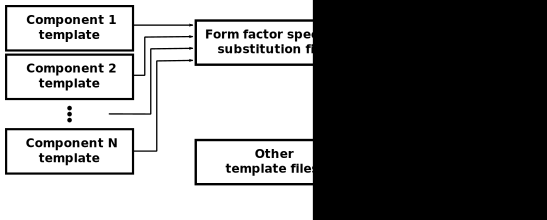
\includegraphics[width=\columnwidth]{./img/templates}
	\caption{Connection between template and substitution files for the EVR.}
	\label{fig:templates}
\end{figure}
Figure~\ref{fig:templates} shows how the templates and substitutions are connected.
\begin{itemize}
	\item 
		\emph{Component templates}~\footnote{evr-base.template, evr-cml.template, evr-in.template, evr-out.template, evr-prescaler.template, evr-pulser.template, sfp.template, ...} contain records corresponding to specific EVR component (eg. inputs, outputs,...). Each EVR form factor supports different components and a different number of each component (exact number of components is available in~\cite{mrm_evr}).
	\item 
		Depending on the EVR form factor, appropriate component templates are listed in a \emph{form factor specific substitution file}.~\footnote{evr-vme-300.substitutions, evr-pcie-300.substitutions, ...}. 
	\item 
		\emph{Form factor specific template files}~\footnote{evr-vme-230.db, evr-pcie-300.db, ...} are are automatically generated uppon build time~\ref{sec:Building from scratch}. These contain all the records for an EVR form factor, as listed in the form factor specific substitution file (eg. records for 2 inputs, 3 prescalers, ...). This template should be included in the EVR substitution file for your IOC application, since it only contains form factor specifics. The application specific behavior can be set using macros. The template accepts macros that define system name, EVR name and macros that define some of the record field values for each component. For example, through setting a correct record field value for a desired output, one can enable or disable this output. Such a template can also be created manually using the MSI tool from a form factor specific substitution file, as described in Section~\ref{sec:Generating templates}.
	\item 
		\emph{Other templates}~\footnote{evr-pulserMap.template, evr-softEvent.template, evr-specialFunctionMap.template, evr-delayModule.template, ...} define application specific behavior and should be included in the EVR substitution file for your IOC application.
\end{itemize}

\section{Building from scratch}\label{sec:Building from scratch}
There are two possible ways to build the mrfioc2 device support. First is using the driver.makefile~\cite{driver.makefile} on the PSI infrastructure, and second using the standard makefile~\cite{appDevGuide}.

\paragraph{Prerequisites}
\begin{itemize}
\item 
	EPICS Base 3.14.x~\cite{epics}.
\item 
	devLib2 2.6~\cite{devlib2}.
\item
	git~\cite{git}, to clone the repository~\cite{git_mrfioc2}.
\item 
	MSI tool~\cite{msi} for expanding databases.
\end{itemize}

\subsection{PSI driver.makefile}\label{sec:PSI driver.makefile}
%driver.makefile~\cite{driver.makefile}, makes it possible to build IOC software projects such as drivers, state notation code, records, etc. with minimal configuration.
To compile to a PSI style module, it is suggested to first clone the PSI git repository for mrfioc2:
\begin{verbatim}
	git clone git@git.psi.ch:epics_drivers/mrfioc2.git
\end{verbatim}
and then:
\begin{enumerate}
\item
	Move to the folder, which contains mrfioc2 sources:
	\begin{verbatim}
		cd mrfioc2
	\end{verbatim}
	
\item 
	Switch to the latest version, which is \texttt{\latestDriverVersion} at the time of writing this manual:
	
	\texttt{git fetch}
	
	\texttt{git checkout \latestDriverVersion}
	
\item
	compile the device support:
	\begin{verbatim}
		make
	\end{verbatim}

\item 
	generate templates:
	\begin{verbatim}
		make db
	\end{verbatim}

\item 
	install the compiled module (mrfioc2 device support and template):
	\begin{verbatim}
		make install
	\end{verbatim}
\end{enumerate}

Compilation will only work on a PSI infrastructure where the correct applications and environment variables are already configured. MSI tool~\cite{msi} is required in order to generate templates. Installed templates should be used for your IOC application, though they can be created separately, following the instructions in Section~\ref{sec:Generating templates}.

Installed module can then be used with one of the example startup scripts~\ref{sec:PSI specifics}.

\subsection{Standard makefile}\label{sec:Standard makefile}
To compile the mrfioc2 as a standard IOC application, it is suggested to first clone the latest mrfioc2 repository from the PSI git: 
\begin{verbatim}
	git clone git@git.psi.ch:epics_drivers/mrfioc2.git
\end{verbatim}

Then follow these steps:
\begin{enumerate}
	\item 
		Move to the folder, which contains mrfioc2 sources:
		\begin{verbatim}
			cd mrfioc2
		\end{verbatim}
		
	\item 
		Switch to the latest version, which is \texttt{\latestDriverVersion} at the time of writing this manual:
		
		\texttt{git fetch}
		
		\texttt{git checkout \latestDriverVersion}
		
	\item 
		Adjust the \texttt{mrfioc2/configure/RELEASE} file for your environment. Make sure that \texttt{DEVLIB2} points to your devLib2 and \texttt{EPICS\_BASE} points to your EPICS base.
	\item 
		Run \texttt{make -f Makefile} in \texttt{mrfioc2} folder.
		\begin{verbatim}
		make -f Makefile
		\end{verbatim}
	\item 
		Template files in \texttt{mrfioc2/Db} folder should be used for your IOC application, though they can be created separately, following the instructions in Section~\ref{sec:Generating templates}.
\end{enumerate}

As mrfioc2 compiles as a standard EPICS application, user can inspect \texttt{iocBoot/iocMrf/} folder for startup script examples.

\section{Generating templates}\label{sec:Generating templates}
As described in Section~\ref{sec:Event Receiver}, the EVR has many form factors with variable number of components. In order to simplify creating IOC applications, a form factor specific template file is generated during the build process.

Whenever possible use the automatic template generation that occurs during the build process!

To create such a template, use a form factor specific substitution file(eg. file list items in ~\ref{sec:mrfioc2 organization:substitution}) and expand it using the
MSI tool~\cite{msi}. The tool works the same way as the EPICS macro substitutions do. The output of
the tool can then be used in the substitution file for your IOC application.

\textbf{However}, in order to set the default values of macros, while
recursively expanding templates (using MSI), a trick is used in the original template files.

\paragraph{Problem}\label{problem}
A VAL record field with a macro might look like this:

\texttt{field( VAL , "\$(MCR=2)")}. 
After using the MSI tool, the field would look like this: 

\texttt{field( VAL , "2")}, 
which means the ability to set the macro value is lost. On the other hand, if the \texttt{\$(MCR)} macro is defined, the default value of the VAL field is lost.

\paragraph{Solution}\label{solution}
The record fields in template files are encapsulated using nested macro, like so:

\texttt{field( VAL , "\$(\$(OBJ)\$(ID)-Div-SP\textbackslash{}=2)")} 
Here is what happens: 
\begin{itemize}
\item 
	\texttt{\$(OBJ)\$(ID)} is extended when running the MSI tool.
This is OK, since it contains template specific information.
\item 
	Notice that `=' is escaped. This means that the MSI tool will only unescape the
default value, instead of applying it to the undefined macro. 
\item  
	Using the MSI tool with macro \texttt{OBJ=PS, ID=0} yields
	
\texttt{field( VAL , "\$(PS0-Div-SP=2,undefined)")} 
\item 
	The macro substitution \texttt{PS0-Div-SP=value} can then be used in our application substitution file to set the field \texttt{value}, otherwise it defaults to `2'.
\end{itemize}

\paragraph{Individual form factor compatible template files} can also be generated. The following \textbf{example} shows how to create a VME-EVR-300 form factor compatible template file, by issuing the following command in \newline\texttt{mrfioc2} folder:

\begin{verbatim}
msi -I evrMrmApp/Db/ -I mrmShared/Db/ 
    -S evrMrmApp/Db/evr-vme-300.substitutions 
    -o evrMrmApp/Db/evr-vme-300.db 
\end{verbatim}

The command will use the EVR form factor specific \newline\texttt{evr-vme-300.substitutions}
file to generate the template \newline\texttt{evr-vme-300.db} to be used in your IOC application substitution file.



%\subsection{Manually generating EVR template}\label{sec:manually-generating-evr-template}
%A MSI tool~\cite{msi} is required to generate a form factor specific template. It
%is recommended to use a predefined template, but you can create one yourself. 
%\texttt{make\_databases.sh} script in \texttt{mrfioc2/PSI} folder is used to generate template files needed for the IOC application The script also copies all the needed templates to the specified location.
%
%\paragraph{make\_databases.sh script usage:}
%\begin{verbatim}
%	./make_databases.sh [options]
%\end{verbatim}
%
%\paragraph{make\_databases.sh script options:}
%\begin{verbatim}
%	-t <top>    ....... Top folder of mrfioc2 (default: ..)
%	-o <output> ....... Output folder for databases (default: ./db)
%	-v          ....... Verbose output (default: no output)
%	-h          ....... Shows options and usage
%\end{verbatim}
%
%\paragraph{Example:} Generate and copy all template files to \texttt{mrfioc2/PSI/db}:
%\begin{verbatim}
%	cd mrfioc2/PSI
%	./make_databases.sh
%\end{verbatim}
%Template files are now available in \texttt{mrfioc2/PSI/db}. There are example substitution files prepared to be used with these templates in \texttt{mrvioc2/PSI}, or you can create your own.



%\section{devlib2}\label{sec:devlib2}
%devLib2~\cite{devlib2} is an extension to the EPICS OS independent VME bus access library (devLib v1) found in the 3.14.x series. The v2 library is an overlay and extension to the v1 library and not a replacement. It is planned that the v2 library will be merged with the v1 library for the 3.15.x series. After that point devlib2 will continue to exist as a location for backports and bug fixes for the 3.14.x series.

%\section{kernel/pcie port}\label{sec:kernel/pcie port}

\section{Firmware update}
\begin{quote}
\textbf{Take great care when flashing the firmware on your device. Wrong bit-files or errors while flashing will most likely render your device unusable!}
\end{quote}
mrfioc2 EPICS device support enables us to update the VME, PCIe and cPCI event generator or event receiver firmware remotely. There are two ways to update the firmware, either through iocsh functions (recommended way) or through EPICS records.


\subsection{Usage of the iocsh functions for accessing the device flash memory} \label{sec:firmware update:iocsh}
In order to read back the content of the flash chip on the device, use the following iocsh command:
\begin{verbatim}
	mrmFlashRead Device File
\end{verbatim}
where:
\begin{itemize}
	\item \texttt{Device} is the device name we wish to read the flash chip memory from. Eg.: EVR0, EVR1, EVG0, EVG1
	\item \texttt{File} is the path to the bit-file where the content of the flash chip memory will be written to.
\end{itemize}

In order to flash firmware to the device, use the following iocsh command:
\begin{verbatim}
	mrmFlashWrite Device File
\end{verbatim}
where:
\begin{itemize}
	\item \texttt{Device} is the device name we wish to flash. Eg.: EVR0, EVR1, EVG0, EVG1
	\item \texttt{File} is the path to the bit-file that contains the firmware we wish to write to the flash chip on the device.
\end{itemize}

Flash chip information and access status can be printed using the following iocsh command:
\begin{verbatim}
	mrmFlashStatus Device
\end{verbatim}
where:
\begin{itemize}
	\item \texttt{Device} is the device name we wish to print the information for. Eg.: EVR0, EVR1, EVG0, EVG1
\end{itemize}

\paragraph{Example:} Reading the information of the EVR0 device flash chip by issuing \texttt{mrmFlashStatus EVR0} command can produce the following output:
\begin{verbatim}
Status report of EVR0 flash chip
    Memory size: 16777216 bytes = 16384 kB = 16 MB
    Sector size: 262144 bytes = 256 kB
    Page size: 256 bytes
    First address for reading / writing is at offset: 0 [bytes]
    Flash is currently not being accessed.
    Last completed flash operation was not successful.
    Last completed read operation was not successful.
\end{verbatim}
The output contains :
\begin{itemize}
	\item basic information about the flash chip (memory, sector and page size),
	\item read / write offset. This is the offset in the flash chip memory, where reading and flashing starts.
	\item Indication whether reading or flashing is currently in progress (either through EPICS records or through iocsh functions).
	\item Indication whether the last completed reading and flashing commands were successful (commands can be issued through EPICS records or through iocsh functions). If no read or write operations were issued yet, the indication states \texttt{not successful}.
\end{itemize}

\subsection{Using EPICS records for accessing the flash memory}
A template file \texttt{flash.template} contains records that expose flash memory access. It be loaded by adding the following lines to the EVR (or EVG) substitution file:
\begin{verbatim}
## Flash access support
## Uncomment this substitution to load records that expose
## read and write access to the flash chip on the device.
#
# Macros:
#  SYS = System name (auto expanded by parent)
#  DEVICE = Event receiver / timing card name (same as mrmEvrSetupVME())
#           Eg. EVR0. (auto expanded by parent)
# 
file "$(mrfioc2_TEMPLATES=db)/flash.template" 
{
	{}
}
\end{verbatim}
When using example substitution file provided for the PSI infrastructure the snippet above is already included, but commented out. In order to use it, uncomment it.
The following records are then available for status reporting:
\begin{itemize}
	\item \texttt{\$(SYS)-\$(DEVICE):Flash-IsOffsetValid-RB} record. Indicates if the offset was set correctly. The offset determines the address on the flash chip where reading/writing starts from/to. It is set automatically based on the device form factor. It can also be set manually through an iocsh command, though this is dangerous. See Section~\ref{sec:firmware update:advanced} for details.
	\item \texttt{\$(SYS)-\$(DEVICE):Flash-InProgress-RB} record. When processed, indicates if reading or flashing is currently in progress (either through records or through iocsh functions).
	\item \texttt{\$(SYS)-\$(DEVICE):Flash-Flash-RB} record. When processed, indicates if the last completed flashing command was successful (flashing command can be issued through EPICS records or through iocsh functions).
	\item \texttt{\$(SYS)-\$(DEVICE):Flash-Read-RB} record. When processed, indicates if the last completed read command was successful (read command can be issued through EPICS records or through iocsh functions).
\end{itemize}

The following procedure enables us to read back the content of the flash chip:
\begin{enumerate}
	\item Check if the offset was set correctly by reading \newline\texttt{\$(SYS)-\$(DEVICE):Flash-IsOffsetValid-RB} record.
	\item Use \texttt{\$(SYS)-\$(DEVICE):Flash-Filename-SP} record to set the path to the bit-file where the content of the flash chip memory will be written to.
	\item Use \texttt{\$(SYS)-\$(DEVICE):Flash-Filename-RB} record to check the previously set path to the bit-file.
	\item Process \texttt{\$(SYS)-\$(DEVICE):Flash-Read-Cmd} record to initiate the reading procedure. 
	\item Periodically process \texttt{\$(SYS)-\$(DEVICE):Flash-InProgress-RB} record in order to see if the procedure has finished. Mind that flash access is slow.
	\item After reading had finished, process \texttt{\$(SYS)-\$(DEVICE):Flash-Read-RB} to see if the operation was successful.
\end{enumerate}

The following procedure enables us to flash the firmware:
\begin{enumerate}
	\item Check if the offset was set correctly by reading \newline\texttt{\$(SYS)-\$(DEVICE):Flash-IsOffsetValid-RB} record.
	\item Use \texttt{\$(SYS)-\$(DEVICE):Flash-Filename-SP} record to set the path to the bit-file that contains the firmware you wish to write to the flash chip on the device.
	\item Use \texttt{\$(SYS)-\$(DEVICE):Flash-Filename-RB} record to check the previously set path to the bit-file.
	\item Process \texttt{\$(SYS)-\$(DEVICE):Flash-Flash-Cmd} record to initiate the flash procedure. 
	\item Periodically process \texttt{\$(SYS)-\$(DEVICE):Flash-InProgress-RB} record in order to see if the procedure has finished. Mind that flash access is slow.
	\item After flashing had finished, process \texttt{\$(SYS)-\$(DEVICE):Flash-Flash-RB} to see if the operation was successful.
\end{enumerate}

\subsection{Advanced} \label{sec:firmware update:advanced}
Sometimes a device with an old, broken or alien firmware needs to be flashed. In these cases the driver will exit with an error, since not all needed parameters could be read from the card. There is an optional \texttt{ignore version error} parameter that can be passed to \texttt{mrmEvgSetupPCI}, \texttt{mrmEvgSetupVME}, \texttt{mrmEvrSetupPCI} or \texttt{mrmEvrSetupVME} commands in order to ignore such errors while setting up the driver. The following startup script\footnote{This is an example for the PSI infrastructure, but the setup command is the same in all cases} example shows the usage of this parameter:
\begin{verbatim}
	require mrfioc2
	
	##########################
	#-----! EVR Setup ------!#
	##########################
	
	mrmEvrSetupVME(EVR0, 3, 0x3000000, 5, 0x26, true);
\end{verbatim}
This startup file will:
\begin{enumerate}
\item Load the latest version of the mrfioc2 driver
\item Setup the VME event receiver using \texttt{mrmEvrSetupVME} command:
	\begin{enumerate}
	\item Set device name to \texttt{EVR0}.
	\item Set VME crate slot to \texttt{3}.
	\item Set the base A32 address (memory offset) to \texttt{0x3000000}.
	\item Set interrupt level to \texttt{5}.
	\item Set interrupt vector to \texttt{0x26}.
	\item Finally, set the optional \texttt{ignore version error} parameter to \texttt{true}.
	\end{enumerate}
\end{enumerate}
When the \texttt{ignore version error} parameter is set (it's value is \texttt{true} or a non-zero number) the device setup procedure will only notify the user of potential version mismatches instead of exiting the driver. Not all parts of the driver are guaranteed to work with \texttt{ignore version error} enabled, but flashing functions described in Section~\ref{sec:firmware update:iocsh} can still be used.

In addition to the flashing functions described in Section~\ref{sec:firmware update:iocsh}, there is another iocsh function that allows us to override the offset from the start of the flash chip memory where reading/writing begins in order to force flashing of the firmware to the device. In normal operation, the offset is auto detected based on the device form factor. The auto detection can fail in rare cases where device firmware is not supported by this driver. This can be the case with old, broken or alien firmwares. \textbf{This is the only case where using this function should be considered.}
\begin{quote}
Setting wrong offset for flashing the device is very dangerous, and should be left to auto detection whenever possible!
\end{quote}
In order to set the offset, use the following iocsh command:
\begin{verbatim}
	mrmFlashSetOffset Device Offset
\end{verbatim}
where:
\begin{itemize}
	\item \texttt{Device} is the device name we wish to flash. Eg.: EVR0, EVR1, EVG0, EVG1
	\item \texttt{Offset} is the offset from the beginning of the flash chip memory to write to / read from.
\end{itemize}


\section{GUI}\label{sec:GUI}
There is a caQtDM~\cite{caqtdm} GUI for the Event Generator and Event Receiver available in \texttt{mrfioc2/evgMrmApp/opi/EVG} and \texttt{mrfioc2/evrMrmApp/opi/EVR}, respectively. These folders contain a script for launching the GUI.

\paragraph{EVR GUI script usage:}
\begin{verbatim}
	./start_EVR.sh -s <system name> [options]
\end{verbatim}


\paragraph{EVR GUI script options:}
\begin{verbatim}
	-d <EVR name> ......... set the event receiver / timing card name 
	                        (default:EVR0)
	-f <form factor> ...... choose the event receiver form factor 
	                        (default: VME)
	                        Choices: VME, PCIe, VME-300
	-h    ................. shows the options and usage
\end{verbatim}


\paragraph{Example:} Open the GUI for the EVR-VME-300 event receiver named \texttt{EVR0}, using system name \texttt{MTEST-VME-EVRTEST}.
\begin{verbatim}
	cd mrfioc2/evrMrmApp/opi/EVR
	./start_EVR.sh -s MTEST-VME-EVRTEST -f VME-300
\end{verbatim}


\bibliographystyle{plain}
\bibliography{references}

\end{document}
